\begin{myprop}
	\iftoggle{eleve}{%
		\kw{Si} deux droites sont \hrulefill 
		
		\vspace*{0.2cm}
		
		\hrulefill
		
		\vspace*{0.2cm}

		\hrulefill		
	}{%
	\kw{Si} deux droites sont perpendiculaires à une même troisième droite, \kw{alors} ces deux droites sont parallèles.
}
\end{myprop}

\vspace*{-0.5cm}

\begin{myex}
	\begin{multicols}{2}
		\iftoggle{eleve}{%		
			\noindent \kw{On sait que} $(d_1)$ et $(d_2)$ sont \hrulefill
			
			\vspace*{0.2cm}
			
			\hrulefill
			
			\vspace*{0.2cm}
			
			\hrulefill
			
			\vspace*{0.2cm}
			
			\hrulefill
			
	}{%
			\noindent \kw{On sait que} $(d_1)$ et $(d_2)$ sont toutes deux perpendiculaires à $(D)$.\\
			\kw{Donc} $(d_1)$ et $(d_2)$ sont parallèles.
		}
			
		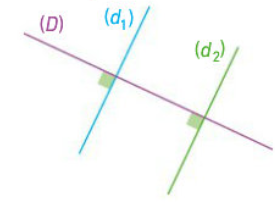
\includegraphics[scale=0.6]{img/para2}
	\end{multicols}
	
\end{myex}


\begin{myprop}
	\iftoggle{eleve}{%	
		\kw{Si} deux droites sont parallèles, \kw{alors} \hrulefill
		
		\vspace*{0.2cm}
		
		\hrulefill

		\vspace*{0.2cm}

		\hrulefill		
	}{%
		\kw{Si} deux droites sont parallèles, \kw{alors} toute perpendiculaire à l’une est perpendiculaire à l’autre
	}
	
\end{myprop}

\vspace*{-0.5cm}

\begin{myex}
	\begin{multicols}{2}
		\iftoggle{eleve}{%		
			\noindent \kw{On sait que} $(d_1)$ et $(d_2)$ sont \hrulefill
			
			\vspace*{0.2cm}
			
			\hrulefill
			
			\vspace*{0.2cm}
			
			\hrulefill
			
			\vspace*{0.2cm}
			
			\hrulefill
			
		}{%
			\noindent \kw{On sait que} $(d_1)$ est parallèle à $(d_2)$ et $(d_1)$ est perpendiculaire à  $(D)$\\
			\kw{Donc} $(d_2)$ est perpendiculaire à $(D)$.	
		}
		
		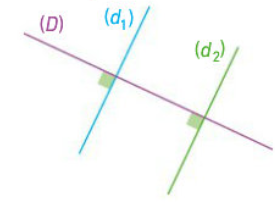
\includegraphics[scale=0.6]{img/para2}
	\end{multicols}
	
\end{myex}

\begin{myprop}
	\iftoggle{eleve}{%
		\kw{Si} deux droites sont parallèles \hrulefill
		
		\vspace*{0.2cm}
		\hrulefill
		
		\vspace*{0.2cm}
		\hrulefill
	}{%
		\kw{Si} deux droites sont parallèles à une même troisième, \kw{alors} ces deux droites sont parallèles entre elles.
	}
	
\end{myprop}

\vspace*{-0.5cm}

\begin{myex}
	\begin{multicols}{2}
		\iftoggle{eleve}{%
			\noindent \kw{On sait que} $(d_1)$ et $(d_2)$ sont \hrulefill
			
			\vspace*{0.2cm}
			
			\hrulefill
			
			\vspace*{0.2cm}
			
			\hrulefill
			
			\vspace*{0.2cm}
			
			\hrulefill
			
		}{%
			\noindent \kw{On sait que} $(d_1)$ et $(d_2)$ sont toutes les deux parallèles à $(d)$\\
			\kw{Donc} $(d_1)$ est parallèle à $(d_2)$.
		}
		
		
		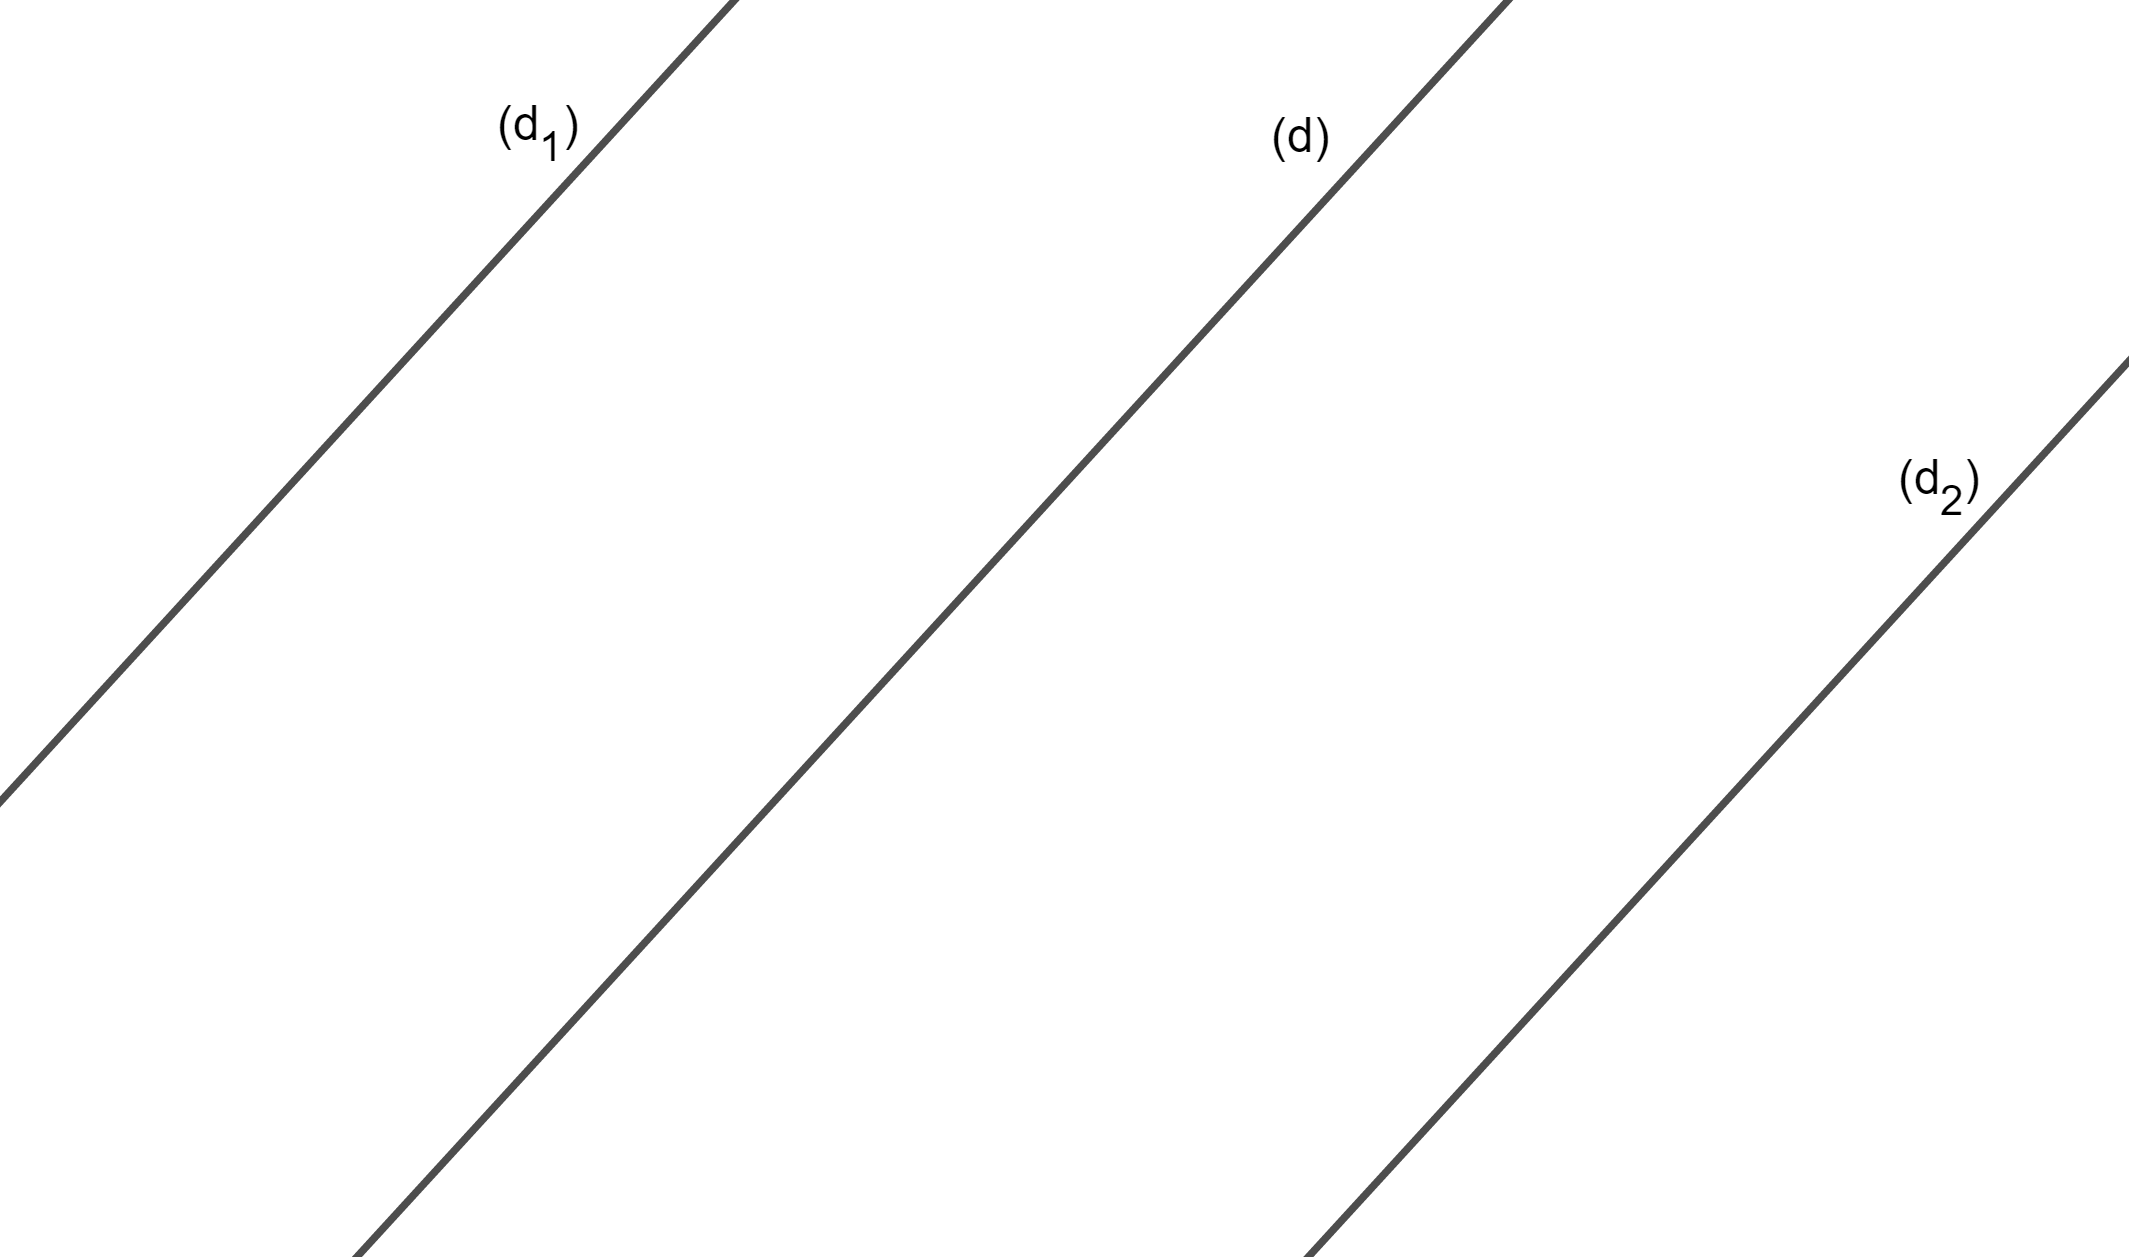
\includegraphics[scale=0.12]{img/para3}
	\end{multicols}
	
\end{myex}
